\documentclass{report}
\usepackage[margin=0.5in]{geometry}
\usepackage{graphicx}

\begin{document}
\Huge
\begin{center}ECSE 548 - VLSI Design \end{center}
\Huge\vspace{1cm}
\begin{center}\textbf{32-Bit Multi-Clock Cycle Multiplier} \end{center}
\Large
\vspace{4cm}
\begin{center} Ibrahim Fakih \end{center}
\begin{center} Yamen Al Samman \end{center}
\vspace{2cm}
\begin{center}
3/12/2013
\end{center}
\newpage
\normalsize
\section*{Introduction}
Although less important than adders, binary multipliers are an important piece of circuitry used in different digital electronics to multiply two binary numbers. They can be found in microprocessors, digital signal processors, and graphic engines. There is a wide range of techniques to build a binary multiplier that vary in performance, energy, complexity and cost. All designs have trade-offs, and are better in one criterion and worse of in another. Most multipliers are designed on the concept of calculating a set of partial products, and then summing the partial products together. 
\\\\
For our VLSI design, we wanted to design a 32-bit multiplier that has the smallest area and least amount of modules. At the same time, we wanted these modules to be easily incorporated into any other application on the chip.

\section*{Design}
The 32-bit multiplier designed for this project is a multi-clock cycle multiplier that includes four main modules (Fig. 1). A 32-bit register to store the multiplicand, a 64-bit shift register to store the product and the multiplier, a 32-bit ALU to perform the additions, and a controller. The 32-bit register used to store the multiplicand is very simple and is designed using flip-flops that have an enable bit.
\\\\
\begin{center} 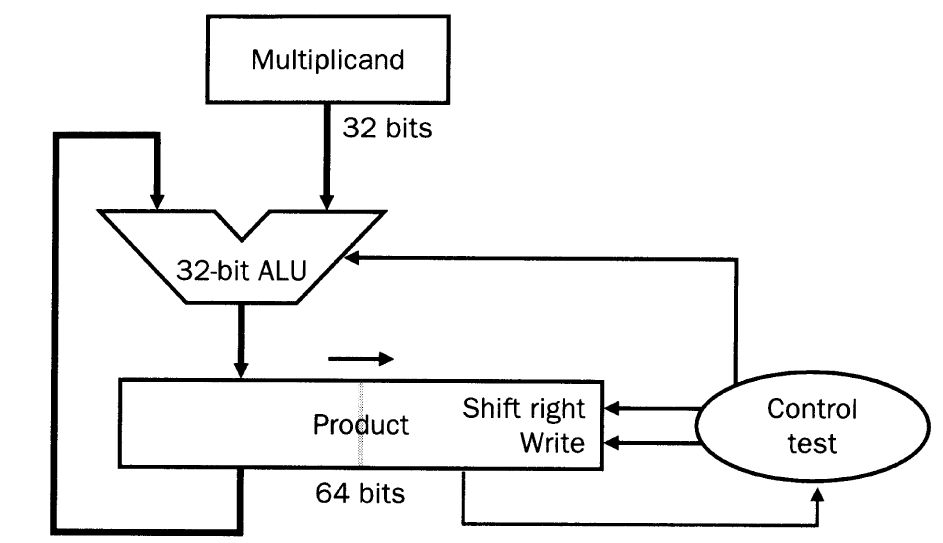
\includegraphics[width=10cm]{MultiClock_schem.png}\end{center}
\begin{center}\bf Fig. 1. Schematic of 32-bit Multi-Cycle Multiplier [1] \end{center}
\noindent
 This design starts of by storing one input in the 32-bit register, while the other gets stored in the lower half of the shift register. The controller then looks at the least significant bit in the shift register, and if it is a one, the ALU adds the multiplicand to the top half of the shift register, while a zero results in no addition. The product register is then shifted by one bit to the right. This repeats for 32 times until the final 64-bit product is stored in the entire shift register.
 \\
 \subsection*{32-bit ALU}
 Although our design can be implemented using a 32-bit adder, an ALU was used instead due to its numerous advantages. ALUs are essential in digital processing and can be found in all microprocessors. Besides  performing simple addition, the ALU can perform logical operations (logical and, and logical or) and integer arithmetics (subtracting and comparing) (Fig. 2(a)). The inclusion of the ALU in our design will make the module usable in other areas and applications of the microprocessors and the possibility of saving area in the final chip design. Another advantage of having an ALU is the possibility of doing signed multiplication if needed without many modifications.
 \\\\
 Although functionalities other than adders are found in the ALU, the 32-bit adder is still the main component of the ALU in terms of area, and its optimization is essential. There are numerous designs for adders that focus on minimizing the critical path which is not important for our design However, the simplest adder in terms of design is the full adder where the output, S = A $\oplus$  B $\oplus$ C and Cout = Maj(A,B,C). Our design optimizes the full adder design to make it more compact and is called the mirror adder. The mirror adder is based on the observation that S can be factored out to use the Cout (S = ABC+ (A +B +C)Cout!). This led our adders to use 28 transistors instead of the usual 32 in normal full adders (Fig. 2(b))[2]. 
 \\\\
 The adders were connected using the simplest design, a Carry Ripple Adder. The critical path delay is from C to Cout, and so the extra delay in computing S is not important and does not affect the performance of the multiplier [2].
 \begin{center} 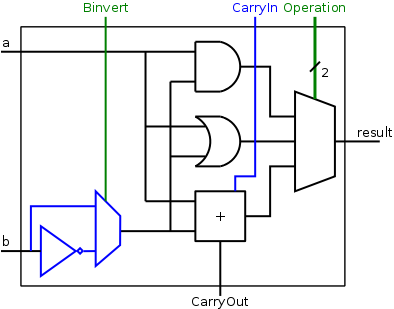
\includegraphics[height=6cm]{Alu_schem.png}	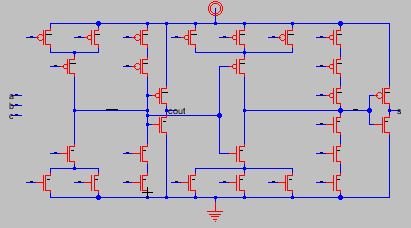
\includegraphics[height=6cm]{adder_schem.png}\end{center}
 \begin{center}\bf Figure 2: (a) Schematic of 32-bit ALU [3] (b) Schematic of Mirror Adder used in the carry ripple adders, carry save adders, and the carry propagate adders. \end{center}
 \subsection*{64-bit Shift Register}
 A 64-bit shift register is required to initially hold the 32-bit multiplier and finally the 64-bit product.  The shift register consists of 64 flip-flops with their inputs connected to multiplexers to choose from the value of the previous flip-flop (with the Most Significant Bit connected to ground) or from parallel load inputs, which are connected to the output of the ALU. The shift registers only performs right-shift as it is the only required function for the multiplier.
  \begin{center} \includegraphics[height=5cm]{shift_schem.png}	\end{center}
  \begin{center}\bf Figure 3: (a) Schematic of a 32-bit Shift Register Module\end{center}
 \subsection*{Controller}
 The controller decides the values of all enable and control signals in the design. As explained previously, 32 repetitions are required to complete the multiplication. Every repetition needs two clock cycles: one for the controller to decide on the next operation and the other for the registers to shift or load values. The Finite State Machine (FSM) of the controller is illustrated in Figure 4 (a).
 Using the state machine, the controller logic was built using a PLA generator used earlier in the semester. A set of flip-flops were used to maintain the state variables outputted from the FSM logic(Fig. 4 (b)).
 \begin{center} 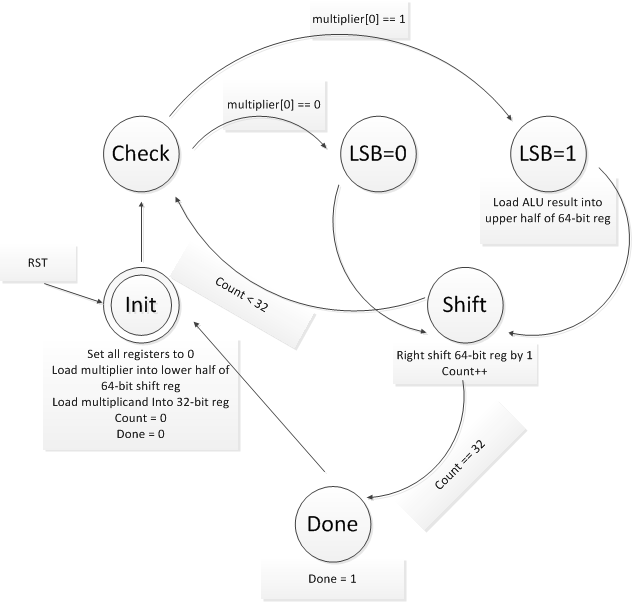
\includegraphics[height=5cm]{controller_state.png}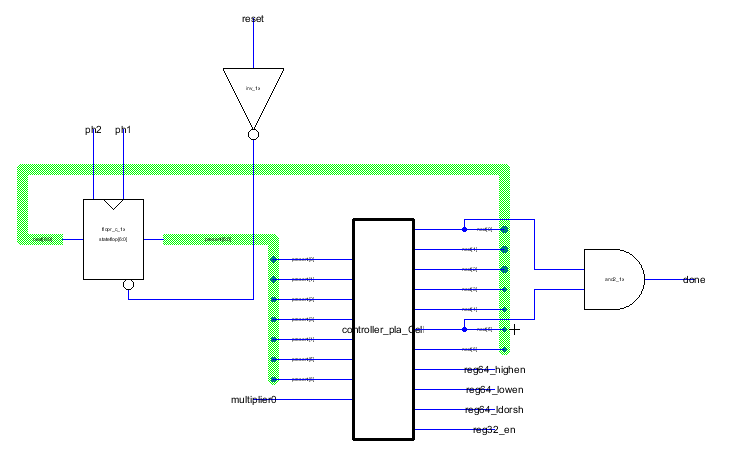
\includegraphics[height=5cm]{controller_schem.png}	\end{center}
   \begin{center}\bf Figure 4: (a) Controller State Diagram (b) Controller Schematic\end{center}
 \section*{Evaluation}
 After completing the design of the multiplier using Electric, it was tested using Electric’s error checks (DRC, ERC, and NCC) which passed successfully. The design was then evaluated by checking if it properly multiplies two 32-bit inputs. Due to the many possible permutation of inputs (over 10\textsuperscript{19}), it was not possible to test them all with the available resources. However, over 10\textsuperscript{11} possible permutations of inputs were tested using ModelSim and the device passed successfully with no errors.
 \\\\
 With the device fully functional, other methods of evaluating the device were looked at. Since our goal was to design a multiplier with least amount of logic, the best way to evaluate the design is to look at the area of the layout(Fig. 5(a)). The multi-clock cycle multiplier has an area of 5,550,000$\lambda$\textsuperscript{2} (3700$\lambda$ x 1500$\lambda$) This includes the white space. 
 \\\\
  However, to evaluate our design, it is important to compare our design with another widely used multiplier, the single-clock cycle multiplier. The single clock cycle multiplier uses an array of carry save adders to compute the partial products, and then carry propagate adders to add the partial products (Fig. 5(b)). Consequently, the 32 single-clock cycle multiplier was built using an array of 32 by 32 carry save adders and 32 carry propagate adders and as a result, speed comes at a cost of area and power. 
 \begin{center}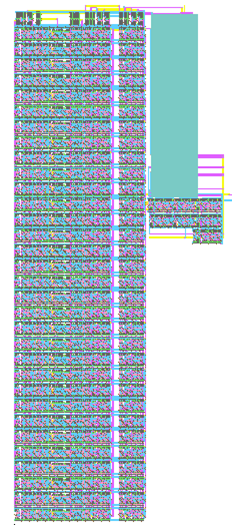
\includegraphics[height=6cm]{MultiClock_lay.png} 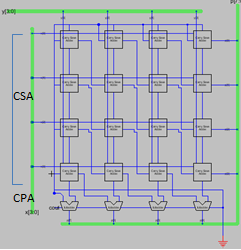
\includegraphics[height=6cm]{singleclock_schem.png}  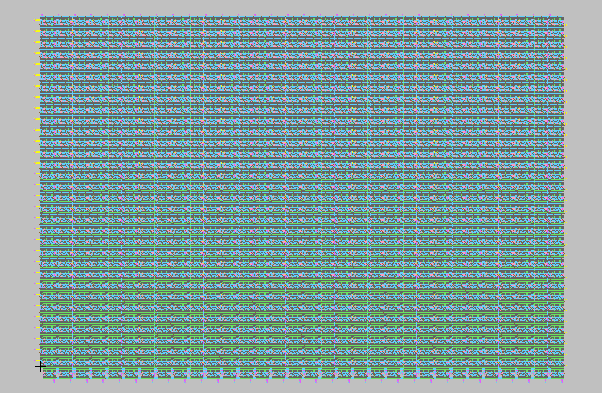
\includegraphics[height=6cm]{singleclock_lay.png}\end{center}
  \begin{center}\bf  Figure 5: (a) Layout of 32-bit Multi-Clock Cycle (b) Schematic of single clock cycle 4-bit multiplier. (c)Layout design of single-clock cycle 32-bit multiplier. \end{center}
  Because of the large array, the single-clock cycle uses a total of 35,712 transistors and has an area of 19,610,000$\lambda$\textsuperscript{2} (3700$\lambda$ x 5300$\lambda$). If registers were included in the design so that the multiplier can store the values for the inputs and the result, the area becomes 22,400,000$\lambda$\textsuperscript{2} (4000$\lambda$ x 5600$\lambda$) which is around 4 times greater than our multi-clock multiplier. 
  \\\\
  Another advantage of the multi-clock cycle multiplier is scalability. Depending on the number of bits being multiplied, the area of the design will be scaled by a factor of n (where n is the number of bits). On the other hand, the single cycle design will be scaled by a factor of n\textsuperscript{2}.
 \\\\
  However, the relative small size of our multiplier design comes at a cost. Although it is five times smaller in size, it takes 64 clock cycles to complete compared to the one clock cycle needed using the carry save multiplier. At the same time, both designs have similar critical paths. The multi-cycle design goes through 32 mirror adders as well as the controller, while the single cycle design goes through 64 mirror adders.
  \section*{Conclusion}
 With the need for multipliers in digital circuitry, we set out at designing a 32-bit multiplier that is aimed at small area processors where size is a constraint. To achieve that, a 32-bit multi-clock cycle multiplier was designed with modules that can be found in a processor (except the controller) and not affect the area greatly. 
 \\\\
 Our multiplier was four times smaller than a single clock cycle multiplier. At the same time, our design can be easily expanded upon using the ALU to include signed multiplication, unlike the single cycle design, which requires significant changes.
 \\\\
 Because area was such an important factor, it was important to consider pitch matching when designing the layouts of the modules. The layouts of the 32-bit register, the ALU and the 64-bit register were made in such a way that they abut together and connect using auto-stitch. This saved considerable amount of space and resulted in a clean design without scattered wires.
 
  
  \section*{Refrences}
  [1] 	Frank Ferrie, "Computer Arithmetics," in ECSE 221, Montreal, McGill, 2010. 
  \\\noindent
  [2] 	Neil West, and David Harris, "Datapath Subsystems," in CMOS VLSI Design - 4th Edition, Pearson, 2009.
  \\\noindent
  [3] 	"Computer Architecture," [Online]. Available: http://cs.nyu.edu/~gottlieb/courses/2007-08-fall/arch/lectures/lecture-04.html. [Accessed 1 Decemeber 2013].
  
  
 
\end{document}